\section{Durchführung}
\label{sec:Durchführung}
\section{Versuchsdurchführung}

Der Aufbau der Schaltungen erfolgt auf einer Steckplatine (Breadboard), wobei der OPV über ei Netzgerät mit einer
symmetrischen Betriebsspannung von $U_S = \pm 15\,\text{V}$ versorgt wird. Zur Signalerzeugung wird ein Funktionsgenerator verwendet.
Zur Analyse der Ein- und Ausgangssignale wird ein digitales Speicheroszilloskops eingesetzt. Dort können Spannungs-Amplituden direkt abgelesen und die Ausschnitte der Spannungskurven als PDF exportiert werden. Ein beispielhafter Aufbau, wie er hier für den Linearverstärker genutzt wurde, ist in \autoref{fig:100} zu sehen. Das Speicherosziloskop ist in \autoref{fig:101} abgebildet. 

\begin{figure}[H]
     \centering
     % Erste Teilgrafik
     \begin{subfigure}[b]{0.45\textwidth}
         \centering
    \caption{Digitales Speicherosziloskop}
    \label{fig:101}
    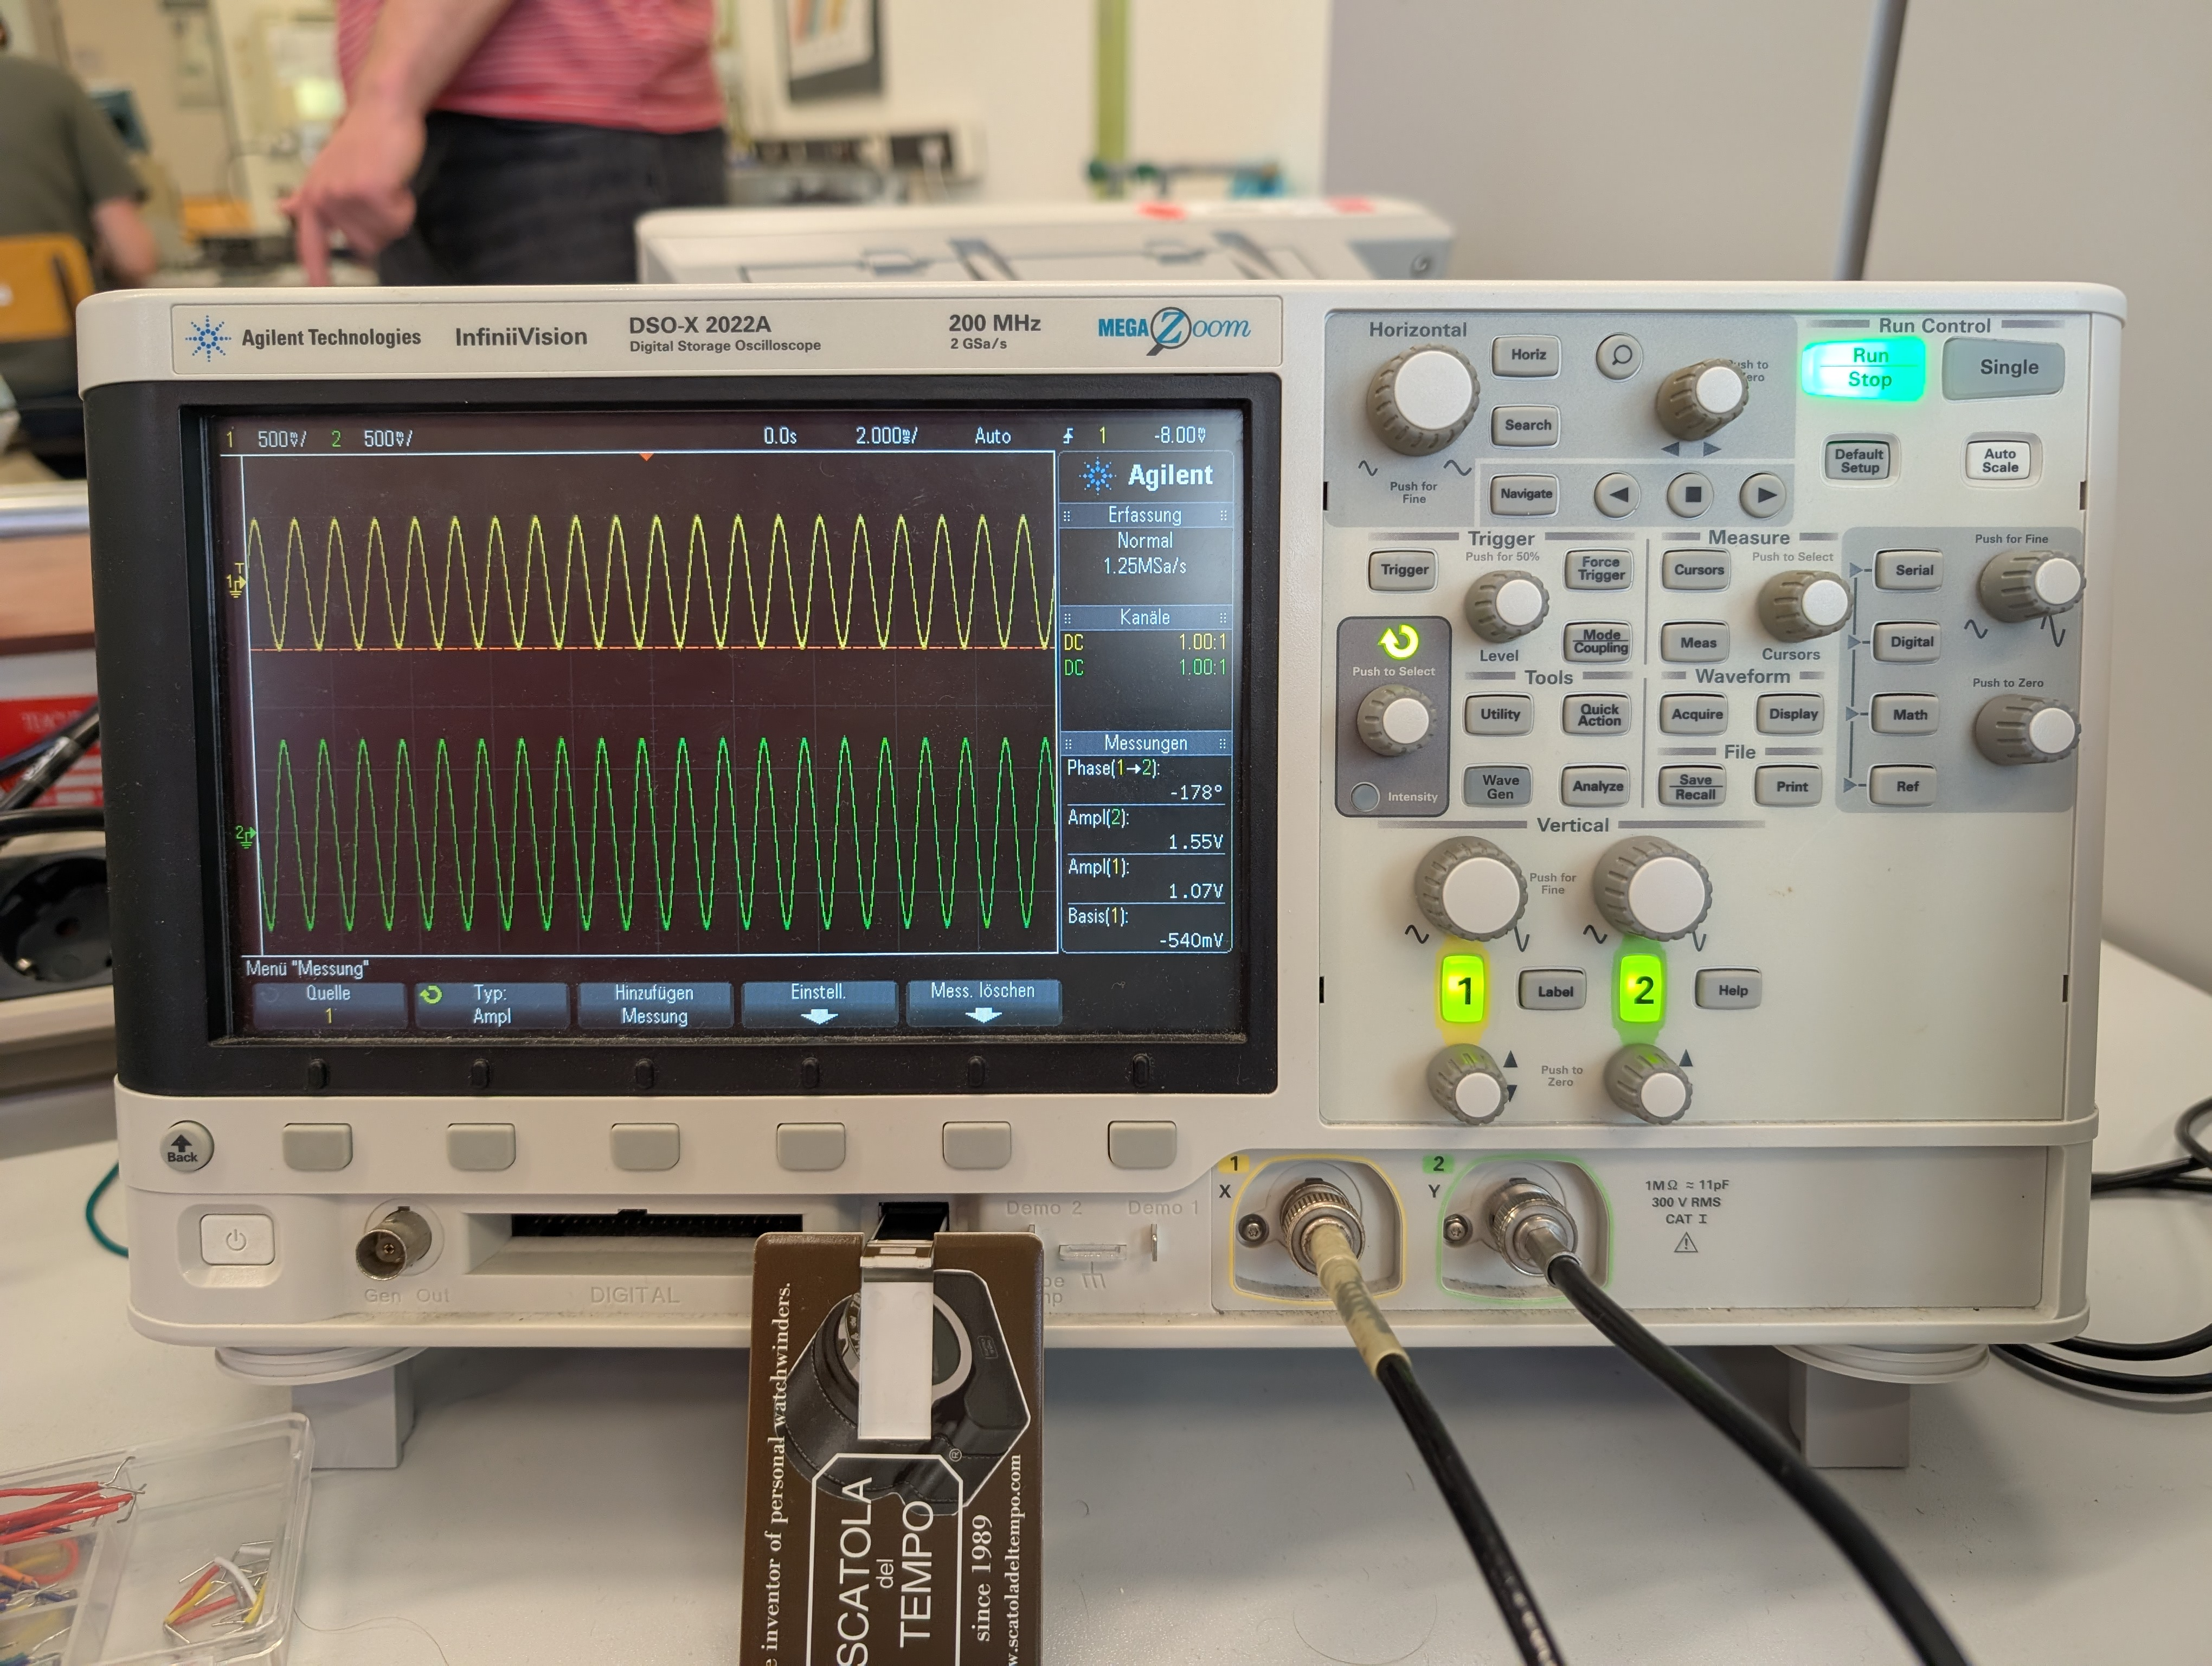
\includegraphics[width=\textwidth]{Bilder/1000040074.jpg}
     \end{subfigure}
     \hfill % Erzeugt horizontalen Abstand zwischen den Bildern
     % Zweite Teilgrafik
     \begin{subfigure}[b]{0.45\textwidth}
         \centering
    \caption{Aufbau Invertierender Linearverstärker}
    \label{fig:100}
    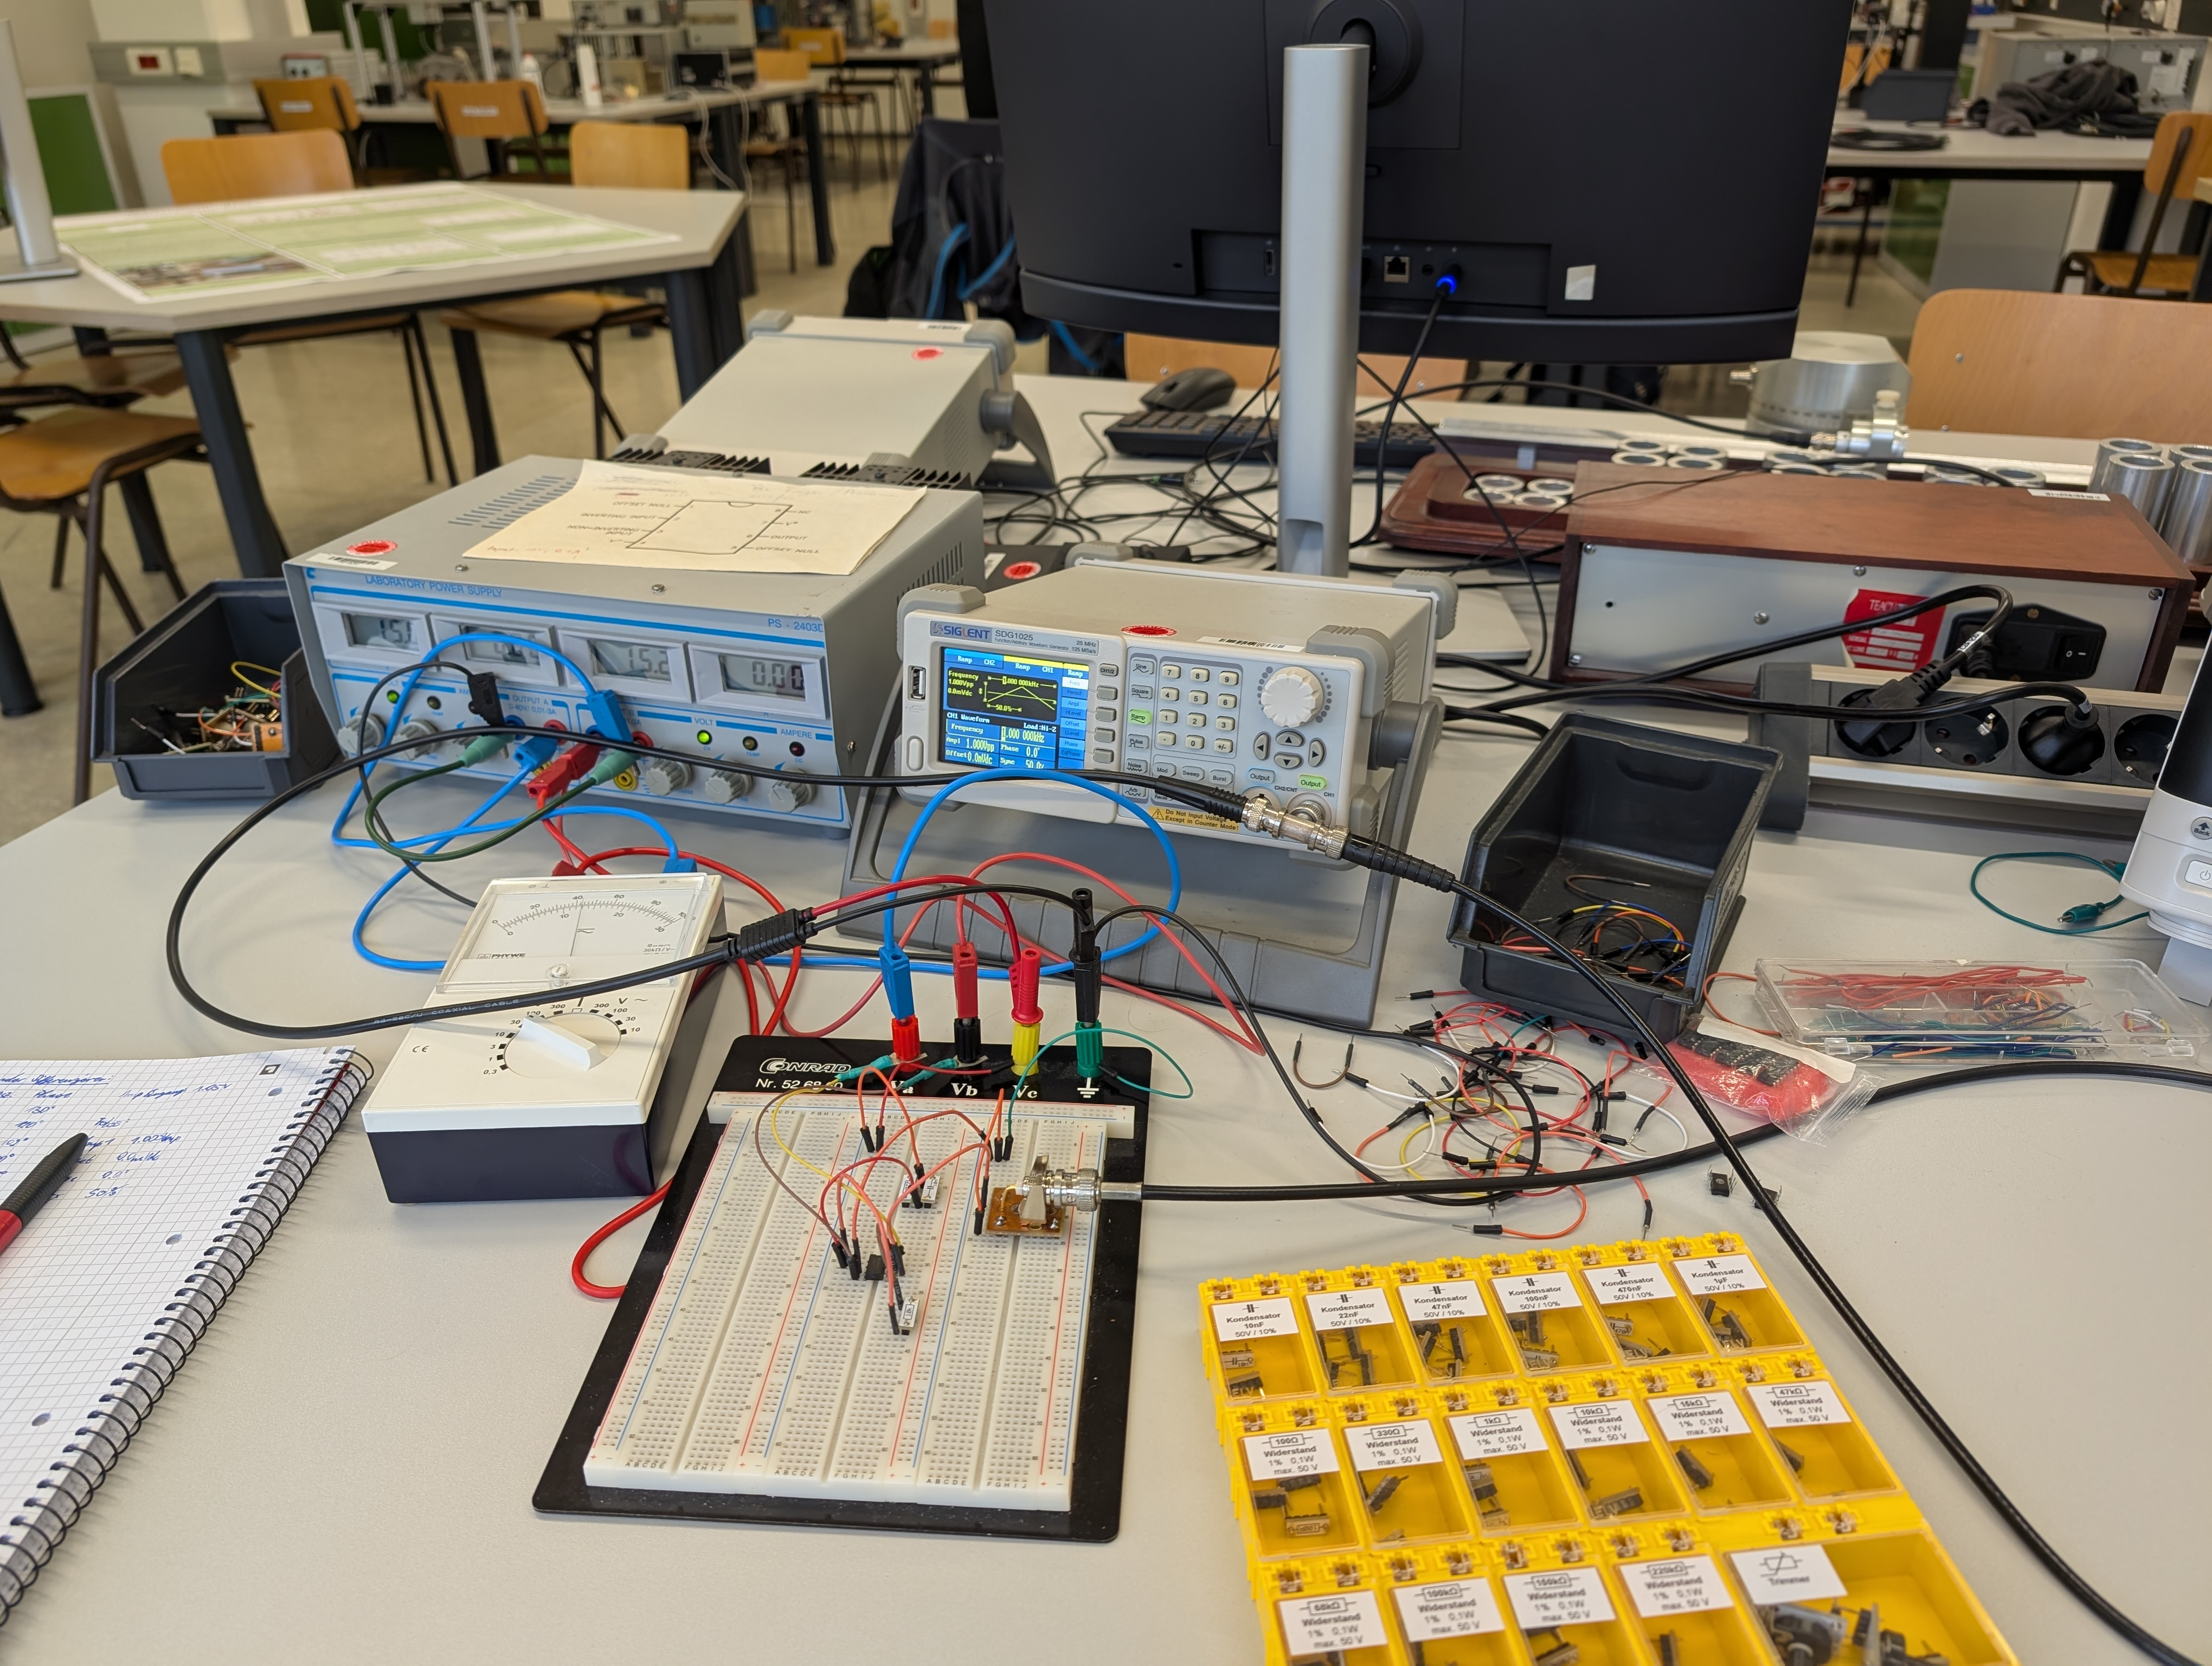
\includegraphics[width=\textwidth]{Bilder/1000040084.jpg}
     \end{subfigure}
     
     \caption{Abbildung 1}
     
\end{figure}

\subsection{Invertierender linearverstärker}

In \autoref{fig:102} ist der Schaltplan für den Invertierenden Linearverstärker zu sehen. Danach wird die schaltung aufgebaut und es werden mit vier unterschiedluchen Wiederstandsverhältnissen, also vier verstärkungsgraden,
\begin{align}
    \frac{R_2}{R_1} = 1.5
    \frac{R_2}{R_1} = 10
    \frac{R_2}{R_1} = 4.7
    \frac{R_2}{R_1} = 3.1
\end{align}
sowie einer Eingangsamplitude von $\qty{1.05}{\volt}$
die frequenzabhängigkeit der Ausgangsspannung des Verstärkers gesucht. Es wird der Frequanzpunkt gesucht, an dem die Ausgangsspannung abfällt.
\begin{figure}[H]
    \centering
    \caption{Schaltung des invertierenden Linearverstärkers \cite{projektlabor_invertierend}}
    \label{fig:102}
    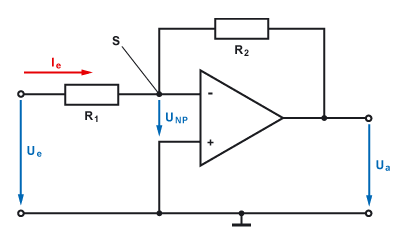
\includegraphics[width=\textwidth]{Bilder/Screenshot_20260511_130927.png}
\end{figure}

\subsection{Umkehr Integrator und invertierender Differenzierer}
Für den Integrierer und Differenzierer wird bis auf einen Unterschied das schaltbild aus \autoref{fig:102} verwendet. Beim Integrierer wird der Wiederstand $R_2$ Durch eine Kapazität $C$ ersetzt. Beim Differenzierer wird der Wiederstand $R_1$ Durch die Kapazität ersetzt. Hierbei soll die Funktion der Schaltung als Integrierer, bzw Differenzierer, verifiziert werden. Dazu Werden als Signalspannungen jewails eine Dreiecks, Rechtecks und sinusspannung angelegt und das Ausgangssignal auf dem Osziloskop Exportiert. 

Die Messungen werden bei einer Eingangsspannung von $\qty{1.05}{\volt}$ sowie einer Frequenz von $f = \qty{1e6}{Hz}$ aufgenommen.

Die Schaltungen für den Integrierer, sowie den Differenzierer sind in \autoref{fig:105} zu sehen.
\begin{figure}[H]
     \centering
     % Erste Teilgrafik
     \begin{subfigure}[b]{0.45\textwidth}
         \centering
         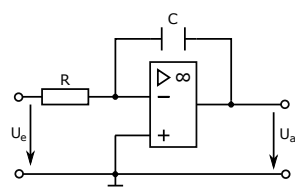
\includegraphics[width=\textwidth]{Bilder/integrator.png}
         \caption{Schltplan zum Integrierer mit der rückgekoppelten Capazität}
         \label{fig:bild1}
     \end{subfigure}
     \hfill % Erzeugt horizontalen Abstand zwischen den Bildern
     % Zweite Teilgrafik
     \begin{subfigure}[b]{0.45\textwidth}
         \centering
         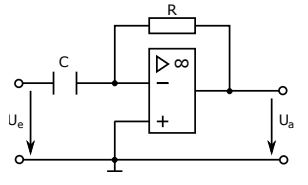
\includegraphics[width=\textwidth]{Bilder/Differenzierer.png}
         \caption{Schltplan zum Differenzierer mit der Capazität am Eingang}
         \label{fig:bild2}
     \end{subfigure}
     
     \caption{Abbildung 1}
     \label{fig:105}
\end{figure}
\subsection{Schmidt-Trigger}nicht-invertierneder 
Es soll die Hysteresekurve der Schmitt trigger Schaltung Aufgenommen werden, dazu wird die Schmidt-Trigger Schaltung aufgebaut und dann die Spannung so lange von null an ins positive variert, bis die Ausgangsspannung in die Sättigung fällt, also bis die Kippspannung erreicht wurde. Daraus lässt sich dann die Hysteresekurve mit positiver und negativer kippspannung konstruieren. 

\begin{figure}
\centering
\caption{Schmidt-Trigger Schaltung}
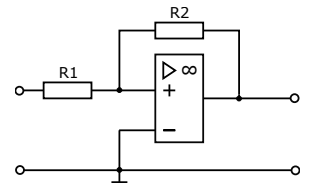
\includegraphics{Bilder/Schmidt.png}
\end{figure}



